\documentclass[ngerman,]{scrartcl}
\usepackage{lmodern}
\usepackage{amssymb,amsmath}
\usepackage{ifxetex,ifluatex}
\usepackage{fixltx2e} % provides \textsubscript
\ifnum 0\ifxetex 1\fi\ifluatex 1\fi=0 % if pdftex
  \usepackage[T1]{fontenc}
  \usepackage[utf8]{inputenc}
\else % if luatex or xelatex
  \ifxetex
    \usepackage{mathspec}
  \else
    \usepackage{fontspec}
  \fi
  \defaultfontfeatures{Ligatures=TeX,Scale=MatchLowercase}
\fi
% use upquote if available, for straight quotes in verbatim environments
\IfFileExists{upquote.sty}{\usepackage{upquote}}{}
% use microtype if available
\IfFileExists{microtype.sty}{%
\usepackage[]{microtype}
\UseMicrotypeSet[protrusion]{basicmath} % disable protrusion for tt fonts
}{}
\PassOptionsToPackage{hyphens}{url} % url is loaded by hyperref
\usepackage[unicode=true]{hyperref}
\hypersetup{
            pdftitle={802.11p - Optimierungsmöglichkeiten},
            pdfauthor={Dominik Bayerl},
            pdfborder={0 0 0},
            breaklinks=true}
\urlstyle{same}  % don't use monospace font for urls
\ifnum 0\ifxetex 1\fi\ifluatex 1\fi=0 % if pdftex
  \usepackage[shorthands=off,main=ngerman]{babel}
\else
  \usepackage{polyglossia}
  \setmainlanguage[]{german}
\fi
\usepackage[]{biblatex}
\addbibresource{bibliography.bib}
\usepackage{graphicx,grffile}
\makeatletter
\def\maxwidth{\ifdim\Gin@nat@width>\linewidth\linewidth\else\Gin@nat@width\fi}
\def\maxheight{\ifdim\Gin@nat@height>\textheight\textheight\else\Gin@nat@height\fi}
\makeatother
% Scale images if necessary, so that they will not overflow the page
% margins by default, and it is still possible to overwrite the defaults
% using explicit options in \includegraphics[width, height, ...]{}
\setkeys{Gin}{width=\maxwidth,height=\maxheight,keepaspectratio}
\IfFileExists{parskip.sty}{%
\usepackage{parskip}
}{% else
\setlength{\parindent}{0pt}
\setlength{\parskip}{6pt plus 2pt minus 1pt}
}
\setlength{\emergencystretch}{3em}  % prevent overfull lines
\providecommand{\tightlist}{%
  \setlength{\itemsep}{0pt}\setlength{\parskip}{0pt}}
\setcounter{secnumdepth}{0}
% Redefines (sub)paragraphs to behave more like sections
\ifx\paragraph\undefined\else
\let\oldparagraph\paragraph
\renewcommand{\paragraph}[1]{\oldparagraph{#1}\mbox{}}
\fi
\ifx\subparagraph\undefined\else
\let\oldsubparagraph\subparagraph
\renewcommand{\subparagraph}[1]{\oldsubparagraph{#1}\mbox{}}
\fi

% set default figure placement to htbp
\makeatletter
\def\fps@figure{htbp}
\makeatother

\usepackage{fancyhdr} \pagestyle{fancy} \usepackage{siunitx}
\usepackage{cleveref}
\usepackage[nohyperlinks, printonlyused, withpage, smaller]{acronym}

\title{802.11p - Optimierungsmöglichkeiten}
\author{Dominik Bayerl}
\date{}

\begin{document}
\maketitle

% pandoc-xnos: cleveref fakery
\newcommand{\plusnamesingular}{}
\newcommand{\starnamesingular}{}
\newcommand{\xrefname}[1]{\protect\renewcommand{\plusnamesingular}{#1}}
\newcommand{\Xrefname}[1]{\protect\renewcommand{\starnamesingular}{#1}}
\providecommand{\cref}{\plusnamesingular~\ref}
\providecommand{\Cref}{\starnamesingular~\ref}
\providecommand{\crefformat}[2]{}
\providecommand{\Crefformat}[2]{}

% pandoc-xnos: cleveref formatting
\crefformat{figure}{fig.~#2#1#3}
\Crefformat{figure}{Figure~#2#1#3}
\crefformat{table}{Tab.~#2#1#3}
\Crefformat{table}{Table~#2#1#3}

\section{3. Optimierungsmöglichkeiten und weitere
Ideen}\label{optimierungsmuxf6glichkeiten-und-weitere-ideen}

Zum derzeitigen Zeitpunkt bestehen noch offene Punkte zur weiteren
Optimierung der Software, die aufgrund des beschränkten zeitlichen
Rahmes des Projektes nicht mehr umgesetzt werden konnten.

Dabei handelt es sich größtenteils um Unschönheiten und
Performance-Maßnahmen in der Software der High-CPU
(Sniffer-Applikation), die jedoch nicht die grundsätzliche Funktion
einschränken. Einige Verbesserungen sollen im Folgenden knapp skizziert
werden.

\subsection{3.1. Optimierung des
IP-Stacks}\label{optimierung-des-ip-stacks}

Der IP-Stack wird immer dann benötigt, wenn ein Paket vom Wireless auf
das LAN-Interface übertragen wird und umgekehrt. Beispielsweise ist es
zur Verpackung der WLAN-Frames notwendig, diese in das RFtap-Format zu
bringen, wobei dieses aus einem UDP-Frame besteht. Derzeit ist dies in
der Datei \texttt{wlan\_mac\_high\_sniffer/rftap.c} als
Chainable-Funktionen implementiert. Dies bedeutet, dass die einzelnen
Bestandteile des Ethernet-Frames stückweise konstruiert und dem Buffer
hinzugefügt werden. Dadurch, dass der Buffer front-alloziert ist (d.h.
es ist lediglich die Start-Adresse und die Länge des Buffers bekannt)
ist es nicht möglich, die Header der Frames direkt dem Beginn des
Buffers hinzuzufügen, da andernfalls der Datenbereich des Frames
überschrieben werden würde. Um dies zu umgehen werden alle Header in
einem separaten Buffer abgelegt und anschließend der Datenteil an das
Ende der Header kopiert (Funktion \texttt{mpdu\_rx\_process()} in
\texttt{wlan\_mac\_high\_sniffer/wlan\_mac\_sniffer.c}). Der
Kopiervorgang ist dabei potentiell ein Performance-Flaschenhals. Die
Notwendigkeit eines einzelnen Buffers der den kompletten Ethernet-Frame
enthält, ergibt sich durch die derzeitige Verwendung des
Ethernet-Interfaces des \ac{fpga} im einfachen \ac{dma}-Modus. Die
tatsächliche Übertragung der Daten auf die Ethernet-Schnittstelle
erfolgt anschließend ohne weitere Beteiligung der CPU durch das
Ethernet-Peripheral.

Im erweiterten \ac{dma}-Modus bietet der Ethernet-\ac{ip-core} die
Möglichkeit der Datenübertragung zur Ethernet-Schnittstelle aus
verschiedenen Speicherbereichen. Dieses Konzept wird bei Xilinx als
``Scatter-Gather-\ac{dma}'' (\emph{grobe Übersetzung}:
Verstreutes-Sammeln-\ac{dma}) bezeichnet
\autocite{xilinx-ethernet-core}. Die Funktionsweise besteht darin, dass
der \ac{dma}-Schnittstelle nicht mehr die Buffer-Adresse und deren Länge
übergeben wird, sondern die Adresse eines sogenannten ``Buffer
Descriptors''. Diese Datenstruktur besteht unter anderem aus der
Buffer-Adresse und einem Längenfeld (siehe
\xrefname{fig.}\cref{fig:dma}). Sobald das \ac{dma}-Peripheral alle
Daten aus dem im Buffer Descriptor referenzierten Buffers übertragen
hat, wird ein Interrupt an die CPU ausgelöst.

\begin{figure}
\centering
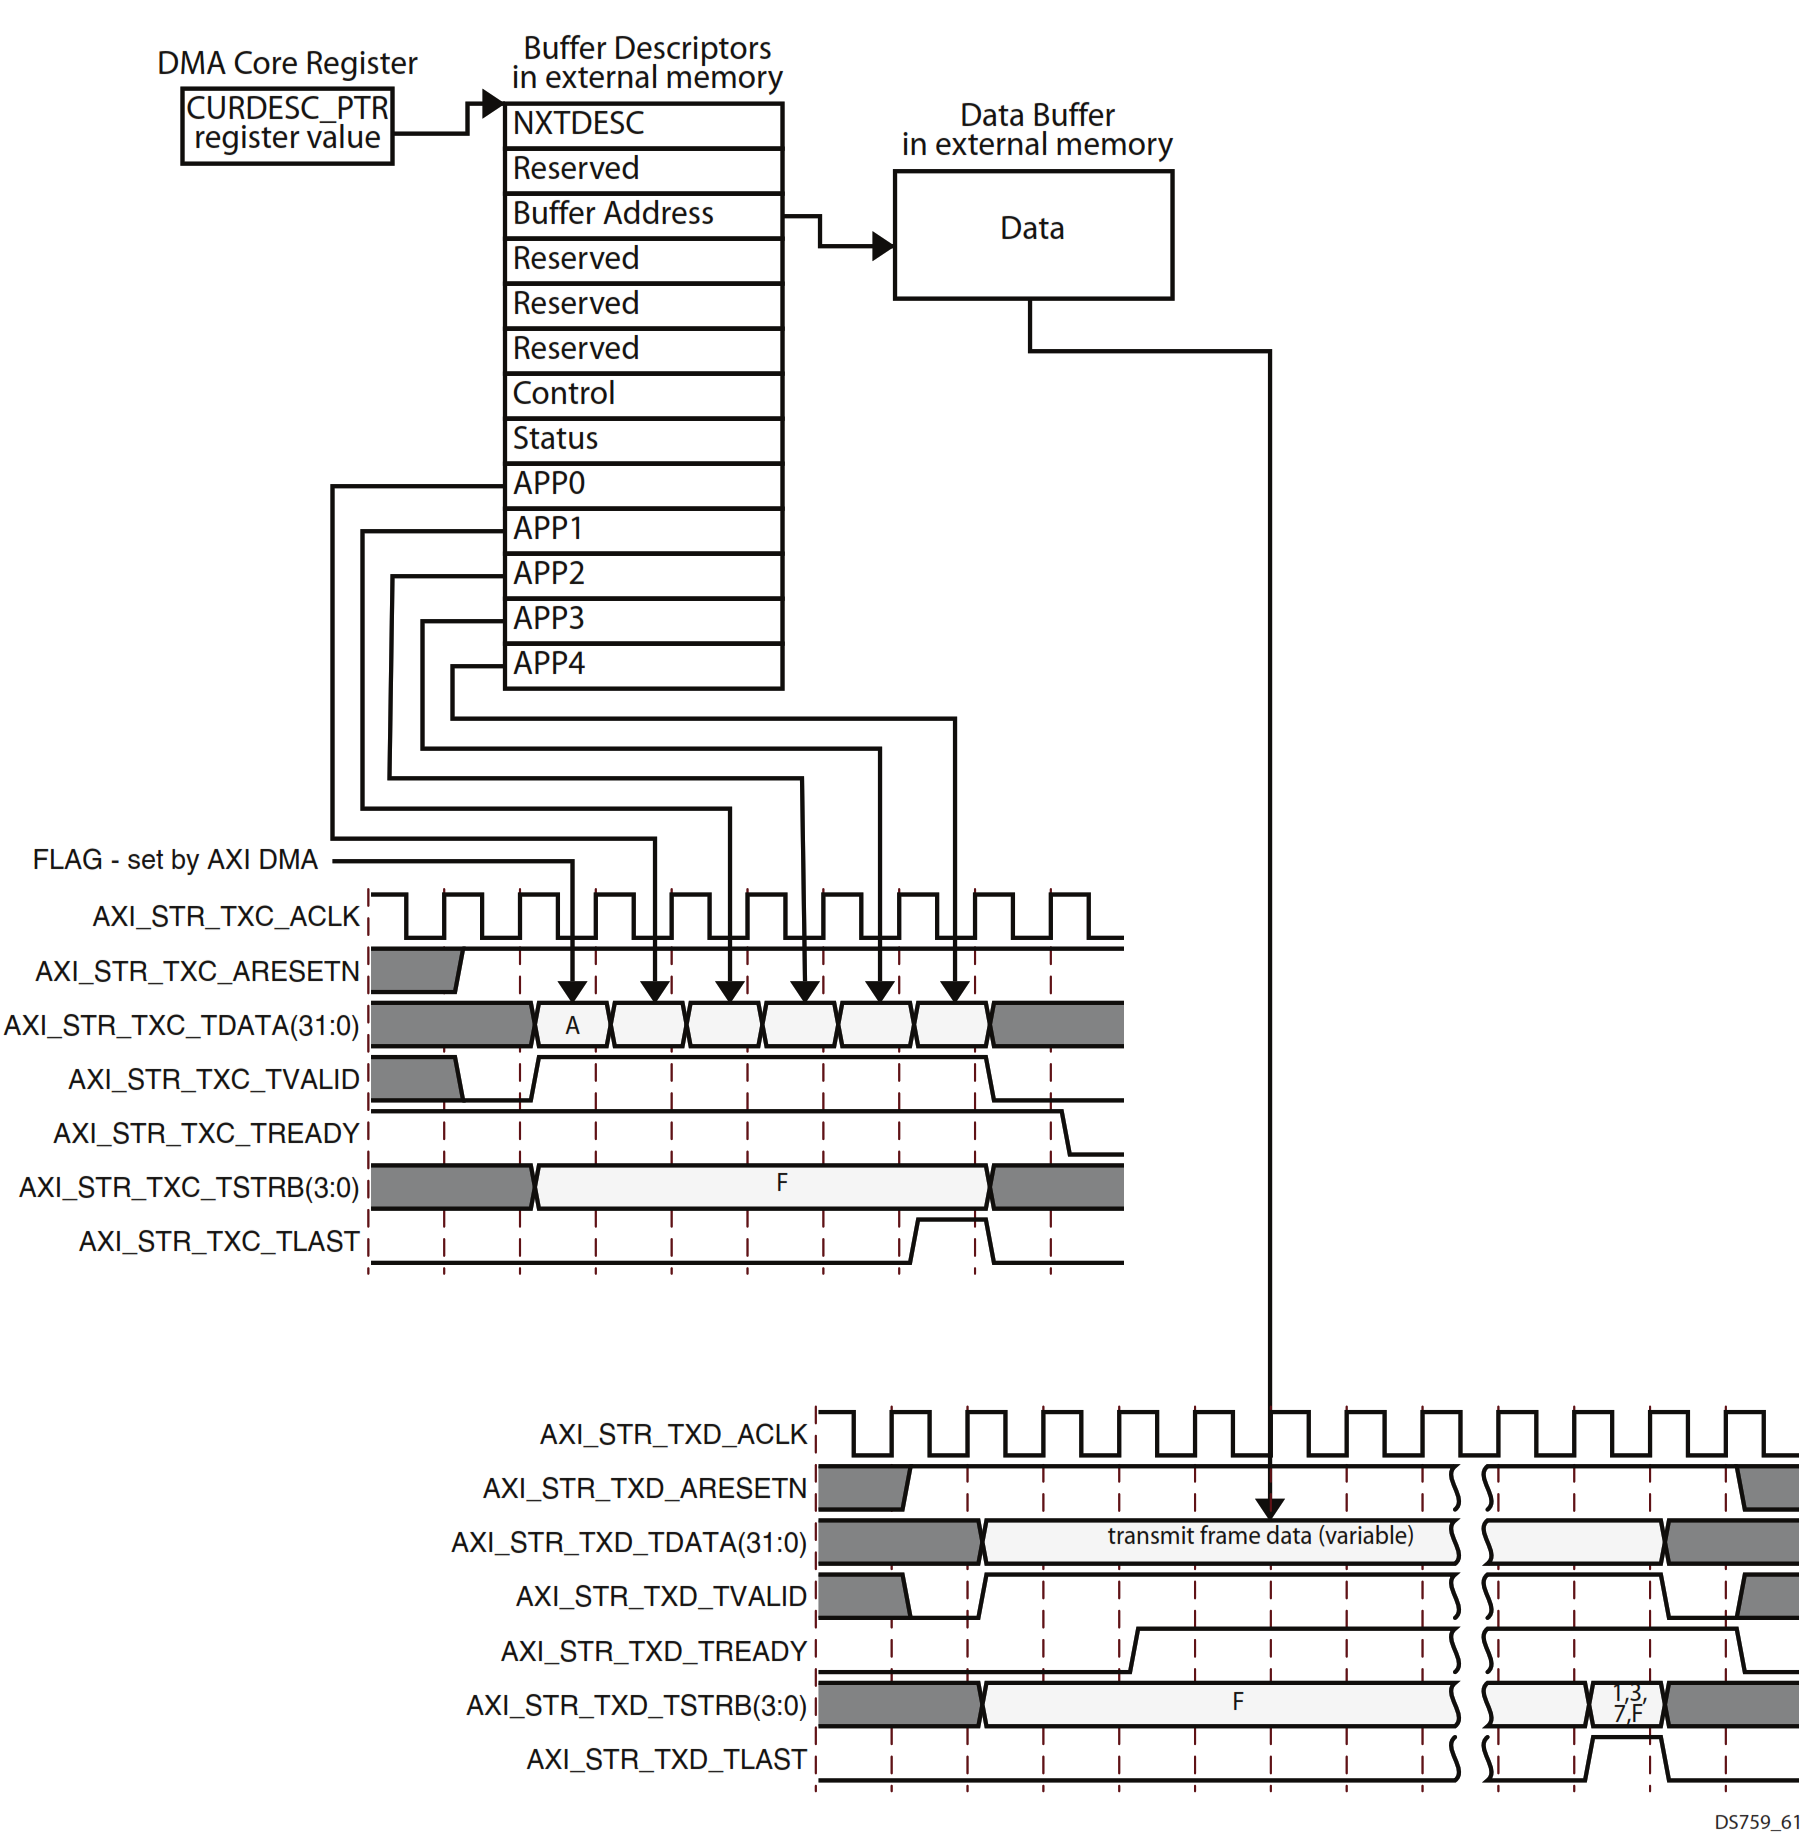
\includegraphics{ds759_axi_ethernet_075.png}
\caption{Xilinx \ac{dma} Buffer
Descriptors\autocite{xilinx-ethernet-core}.\label{fig:dma}}
\end{figure}

Der Vorteil dieses Verfahrens besteht darin, dass eine zweite
Indirektionsschicht eingeführt wird; dadurch ist es nicht mehr
notwendig, dass sämtliche \ac{dma}-Daten sequentiell im Speicher liegen.
Üblicherweise implementiert man dazu eine Single-Linked-List (\ac{fifo}
Queue) aus Buffer-Descriptors, die nach jedem \ac{dma}-Interrupt
weitergeschalten wird. Für den konkreten Fall der Ethernet-Frames
ermöglicht dieses Verfahren, die einzelnen Header-Bestandteile
unabhängig im Speicher ablegen zu können. Dadurch ist ein echter
Zero-Copy Modus - also ohne Daten kopieren zu müssen - möglich.

\subsection{\texorpdfstring{3.2. Nutzung der
\ac{cfo}-Estimates}{3.2. Nutzung der -Estimates}}\label{nutzung-der--estimates}

Im Empfangspfad des WARPv3 existiert bereits ein Block zur Korrektur
eventuell vorhandener Frequenzabweichungen der Sender bzw. des
Empfängers (\textbf{TODO}: Referenz Aufbau Reference Design). Dabei wird
mittels des \ac{lts}-Feldes über mehrere Frames die Frequenz des
empfangenen Signals gegenüber der Center-Frequenz des gewählten Channels
bestimmt und anschließend zur Korrektur der Fourier-Transformation der
einzelnen Carriers genutzt.

In den meisten kommerziellen WiFi-Transceivern wird die Informationen
anschließend verworfen, da sie für die darüberliegende Schicht (Layer 2,
MAC Layer) nicht benötigt wird. Nicht so im WARP Reference Design: die
geschätzte \ac{cfo} wird durch die Low-CPU an die High-CPU in der
Methode \texttt{mpdu\_rx\_process()} in der Datei
\texttt{wlan\_mac\_high\_sniffer/wlan\_mac\_sniffer.c} als Feld
\texttt{cfo\_est} der Struktur \texttt{rx\_frame\_info\_t} übergeben.
Gleichermaßen wird die Information bereits durch die Sniffer-Applikation
in den RFtap-Frames an die Ethernet-Schnittstelle übertragen (\emph{Flag
3, Frequency offset field is present}). Dies ermöglicht die Auswertung
der \ac{cfo}-Estimates beispielsweise im Wireshark eines angeschlossenen
Computers.

Die Information ist besonders deswegen interessant, da sie (unter
anderem) für zwei Anwendungsfälle genutzt werden kann, die im Folgenden
dagelegt werden sollen:

\subsubsection{3.2.1. Doppler-Effekt}\label{doppler-effekt}

Wie jedes elektromagnetische Signal unterliegen auch die 802.11p-WLAN
Signale dem Doppler-Effekt. Dieser besagt, dass ein Signal der Frequenz
\(f_S\) das von einem Sender \(S\) an einen Empfänger \(B\) derart
übertragen wird, dass Sender und Empfänger eine Relativgeschwindigkeit
\(v_S - v_B = v \neq 0\) besitzen, beim Beobachter eine
Frequenzabweichung
\(f_{B} = \frac{f_{S}}{\gamma} = f_{S} \sqrt{1-\frac{v^2}{c^2}} \approx f_{S} \left(1 - \frac{v^2}{2c^2}\right)\)
erfährt.

Diese Frequenzabweichung muss durch den Empfänger detektiert und
kompensiert werden. Für die Anwendung WLAN wird dies durch die Korrektor
der \ac{cfo} übernommen. Hat ein Empfänger nun Kenntnis über den
statischen \ac{cfo} (bedingt durch ungenaue Oszillatoren) eines Senders,
kann er durch die Messung des aktuellen \ac{cfo} eine dynamische
Frequenzabweichung bestimmen, bei der der Doppler-Effekt eine nicht
unerhebliche Rolle spielt. Für 802.11p bedeutet dies, dass zwei
Fahrzeuge, die miteinander im Funkkontakt stehen, ihre gegenseitige
Relativgeschwindigkeit ohne Zusatzhardware über die WLAN-Schnittstelle
bestimmen könnten. Dies ermöglicht eine Reihe weiterer Funktionen, wie
Notbremsassistenten, Adaptive Tempomaten und ähnliches.

\subsubsection{3.2.2. PHY-Fingerprinting}\label{phy-fingerprinting}

In einer separaten Teilgruppe des Projektes wurde ein Verfahren zur
Manipulation von Funknetzen, sog. MAC-Spoofing und Evil-Twin-APs
evaluiert. Die Verfahren basieren darauf, dass die Merkmale die zur
Identifikation der Funkteilnehmer verwendet werden, sehr leicht
manipulierbar sind (MAC-Adresse bzw. SSID/BSSID). Für nicht weiter
kryptographisch gesicherte Netzwerke (Offene WLANs) stellen diese
Attacken ein erhebliches Sicherheitsrisiko dar, da dadurch eine Reihe
weiterer Angriffe (Man-in-the-middle, Phishing, ARP-Spoofing, \ldots{})
ermöglicht werden.

Das Mango-Board bietet gegenüber kommerzieller WLAN-Hardware die
Möglichkeit, sämtliche Parameter der Funkübertragung zu erfassen,
insbesondere auch die des physikalischen Layers, beispielsweise in Form
der Center-Frequency-Offsets. Diese Parameter sind unabhängig von den
gesendeten Daten, sondern werden ausschließlich durch die
RF-Charakteristik der Hardware des Senders beeinflusst und eignen sich
dadurch als Merkmal zur Identifikation eines einzelnen Sende-Moduls.
Durch ein geeignetes Fingerprinting-Verfahren über mehrere verschiedene
Merkmale (\ac{cfo}-Estimates, Signal-Power, Noise-Power) kann dadurch
eine Zuordnung anderer Merkmale (MAC-Adresse, SSID) zu einem
physikalischen Sender geschaffen werden. Dadurch wird es ermöglicht,
oben genannte Angriffe erkennen zu können, da im Falle eines vorhandenen
Angreifers zwei verschiedene Sendemodule (mit unterschiedlichen
Fingerprints) die selben High-Level Merkmale (MAC-Adresse, SSID) nutzen
würden.\autocite{rftap-mac}

\subsubsection{3.2.3. Linux Kernel}\label{linux-kernel}

Im Verlauf des Projekts zeigte sich, dass der Ansatz des 802.11
Reference Designs als Bare-Metal Software (d.h. ohne Betriebssystem)
mehrere Schwächen besitzt: eine Iteration der entwickelten Software
bedingt stets eine komplette Neuprogrammierung des \ac{fpga}-Designs.
Desweiteren ist es nicht ohne weiteres möglich, Konfigurationsparameter
(Channel, Baseband, \ldots{}) während des Betriebs anpassen zu können.
Diese Funktion wurde zwar rudimentär über eine UART-Konsole eingebaut,
hat jedoch Schwächen in der Bedienbarkeit und Robustheit.

Weitere fehlende bzw. nur im Ansatz vorhandene Funktionen sind eine
Debugging-Schnittstelle (\texttt{xil\_printf()} über die UART-Konsole),
ein Scheduler (Scheduling auf der CPU-High implementiert, non-preemptive
round-robin mit Auflösung im Millisekunden-Berich) und die Möglichkeit
zur Nutzung der von Xilinx bereitgestellten Peripheral-Treiber
(insbesondere die Ethernet-Schnittstelle).

Diese offenen Punkte können durch den Einsatz eines Betriebssystems
gelöst werden. Xilinx bietet bereits einen an die MicroBlaze-Architektur
angepassten Linux Kernel \autocite{xilinx-microblaze} an. Zusätzlich
sind für die meisten \ac{ip-core} Linux-Treiber vorhanden, die einfach
integriert werden können \autocite{xilinx-linux-drivers}.

Ungelöst ist dabei die Problematik der Treiber für benutzerdefinierte
Peripherals - insbesondere für die \emph{radio\_controller}, die
zentraler Bestandteil des WARP Reference Designs sind. Hier ist eine
Anpassung der standalone-Treiber an die Schnittstelle des Linux-Kernels
notwendig.

\printbibliography

\section*{Abkürzungsverzeichnis}\begin{acronym}[ip-core]
\acro{cfo}[CFO]{Center Frequency Offset}
\acro{dma}[DMA]{Direct Memory Access}
\acro{fpga}[FPGA]{Field Programmable Gate Array}
\acro{fifo}[FIFO]{First in First out}
\acro{ip-core}[IP-Core]{Intellectual Property Core}
\acro{lts}[LTS]{Long training sequence}
\acro{pll}[PLL]{Phase-locked Loop}
\acro{rf}[RF]{Radio Frequency}
\end{acronym}

\end{document}
